% Part: set-theory
% Chapter: ordinals
% Section: idea

\documentclass[../../../include/open-logic-section]{subfiles}

\begin{document}

\olfileid{sth}{ordinals}{idea}
\olsection{ক্রমসংখ্যার সাধারণ ধারণা}

স্বাভাবিক সংখ্যাগুলিকে তাদের প্রচলিত ক্রমে দেখি:
\begin{center}
	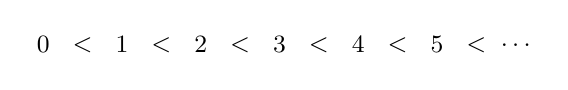
\begin{tikzpicture}
	\foreach \x/\xtext in {0, 1, 2, 3, 4, 5}
	{
		\node (\x a) at (\x, 1) {\small{$\x$}};
		\node (\x a) at (\x.5, 1) {\small{$<$}};
	}
	\node (ldots) at (6, 1) {\small{$\ldots$}};
	\end{tikzpicture}
\end{center}
প্রযুক্তিগত ভাষায় একে $\omega$-অনুক্রম বলি।
বস্তুত, সেট-ক্রমধারার পর্যায়গুলি নিয়ে প্রথম যে
নির্মাণ করেছিলাম, তাতেও এই সাধারণ ক্রম প্রতিফলিত।
কিন্তু এখন ধরি, এই অনুক্রমে $0$-কে শেষে সরিয়ে দিলাম,
যাতে এটি অন্য সব সংখ্যার পরে আসে:
\begin{center}
	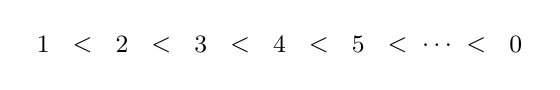
\begin{tikzpicture}
	\foreach \x/\xtext in {1, 2, 3, 4, 5}
	{
		\node (\x a) at (\x, 1) {\small{$\x$}};
		\node (\x a) at (\x.5, 1) {\small{$<$}};
	}
	\node (ldots) at (6, 1) {\small{$\ldots$}};
	\node (bea) at (6.5, 1) {\small{$<$}};
	\node (noa) at (7, 1) {\small{$0$}};
	\end{tikzpicture}
\end{center}
এখানে বস্তুগুলি একই, কিন্তু তাদের ক্রম মৌলিকভাবে
আলাদা: প্রথম ক্রমের কোনো শেষ সদস্য ছিল না; নতুন
ক্রমের আছে। আসলে নতুন ক্রমে প্রথমে বস্তুগুলির একটি
$\omega$-অনুক্রম ($1, 2, 3, 4, 5, \ldots$), তারপর
আরেকটি বস্তু আছে। তাই এটি একটি $\omega+1$-অনুক্রম।

এই একই বস্তুগুলি দিয়ে আরও নানা ধরনের ক্রম বানানো
যায়। যেমন, প্রথমে সব জোড় সংখ্যা (স্বাভাবিক ক্রমে),
তারপর সব বিজোড় সংখ্যা (স্বাভাবিক ক্রমে) নিই:
\begin{center}
	\begin{tikzpicture}
	\node(a1) at (1,1) {\small{$0$}};
	\node(a2) at (1.5,1) {\small{$<$}};
	\node(a3) at (2,1) {\small{$2$}};
	\node(a4) at (2.5,1) {\small{$<$}};
	\node(a5) at (3,1) {\small{$4$}};
	\node(a6) at (3.5,1) {\small{$<$}};
	\node(dots) at (4,1) {\small{$\ldots$}};
	\node(aaoe) at (4.5,1) {\small{$<$}};
	\node(b1) at (5,1) {\small{$1$}};
	\node(b2) at (5.5,1) {\small{$<$}};
	\node(b3) at (6,1) {\small{$3$}};
	\node(b4) at (6.5,1) {\small{$<$}};
	\node(b5) at (7,1) {\small{$\ldots$}};
	\end{tikzpicture}
\end{center}
এটি একটি $\omega$-অনুক্রমের পরে আরেকটি
$\omega$-অনুক্রম; অর্থাৎ $\omega+\omega$-অনুক্রম।

এভাবে আরও এগোনো যায়। কিন্তু আমরা চাই এই
\emph{ক্রমগুলি} নিয়ে কথাবার্তা বোঝার একটি সাধারণ
পদ্ধতি।

\end{document}
